\documentclass[../../main.tex]{subfiles}
    
    \lstset{basicstyle=\small,
      showstringspaces=false,
      commentstyle=\color{black},
      keywordstyle=\color{blue}
    }
    
    \graphicspath{{images/Kran/}{../../images/Kran/}}

    \begin{document}
    \subsection{Würfelaufnahme/Transport}
         Um den Würfel rechts neben der Gleisstrecke aufzunehmen wird eine einfache Lösung angestrebt, steuerungstechnisch sowie mechanisch. Aus dem morphologischen Kasten (Anhang) und der Nutzwertanalyse geht hervor, dass die Würfelaufnahme mit einem Draht und einem Stab durchgeführt wird. Damit nur ein Aktor angesteuert werden muss wird von dem Prinzip einer Kurvenscheibe Gebrauch gemacht.  Die gesamte Vorrichtung besteht grundsätzlich aus drei Elementen. Einem Kran zur Lastaufnahme, einem Antriebsstrang und der Kurvenscheibe.

        \begin{figure}[H]
            \centering
            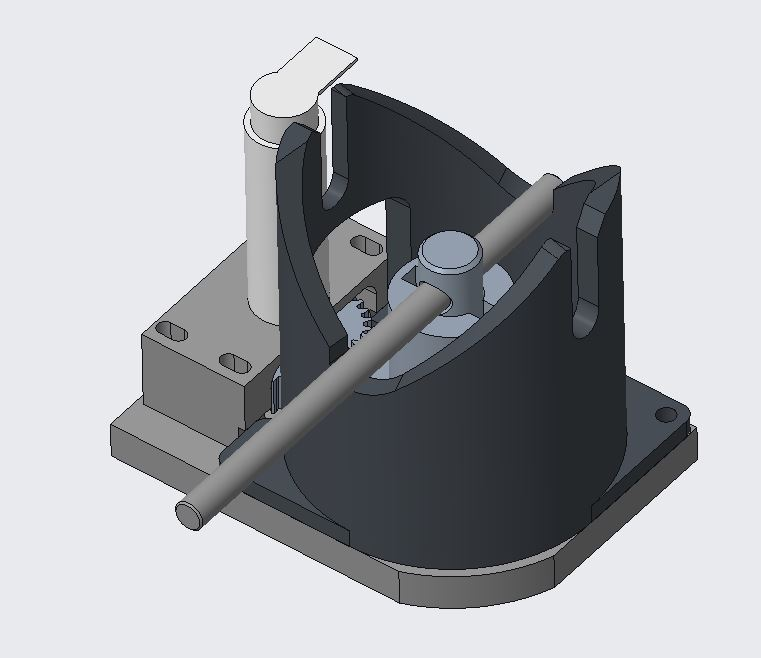
\includegraphics[width=0.8\textwidth]{../../images/Kran/BG.JPG}
            \caption {Baugruppe}
            \label{fig:et_komponenten}
        \end{figure}

    \subsubsection{Kran}
         Der Kran besteht aus drei Drehteilen, welche mit einer Pressverbindung zusammengefügt wurden. Das zentrale Element des Krans wird auf Grund seiner optimalen Gleiteigenschaften und der geringen Dichte aus Teflon gefertigt. Der kleinere Stahlstift ist für die Drehmomentübertragung zuständig. Der Grössere der beiden Stahlstifte ist der eigentliche Ausleger. An dessen ende wird ein Draht aus Federstahl geformt und angehängt. Dieser Draht soll als Haken zur Lastaufnahme dienen. Weiter ist der Ausleger in beide Richtungen von der Drehachse ausgedehnt, da die Kurvenscheibe zwei Laufflächen hat, um für einen stabilen Hub zu sorgen. Der ganze Aufbau wird mittels einer Spielpassung in einer Bohrung mit zwei längsnuten in einem 3D gedruckten, modifizierten Zahnrad gelagert.  

        \begin{figure}[H]
            \centering
            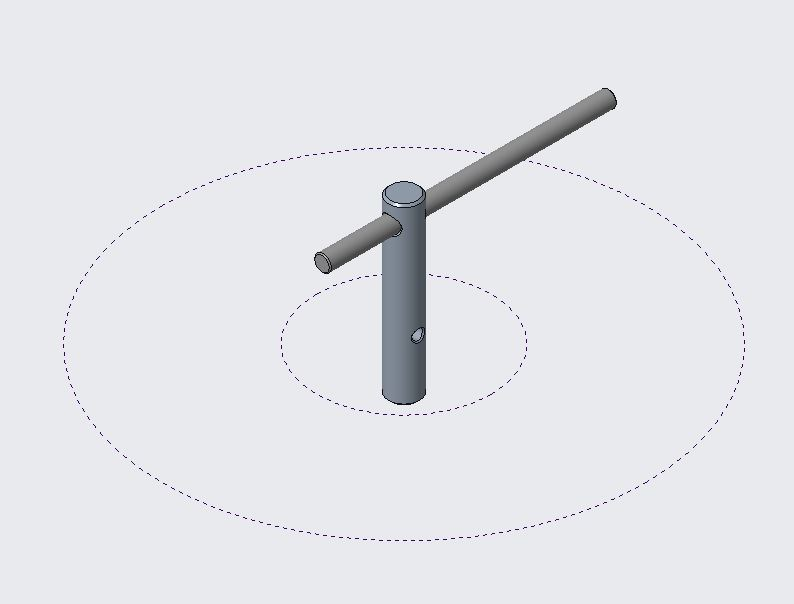
\includegraphics[width=0.5\textwidth]{../../images/Kran/Top.JPG}
            \caption {Draufsicht}
            \label{fig:et_komponenten}
        \end{figure}



    \subsubsection{Antriebsstrang}
        Der Antrieb besteht aus einem Motor, dessen Aufhängung und zwei Zahnrädern. Der Motor ist ein bürstenbehafteter Motor mit Encoder und Getriebe vornedrauf. Mit dieser Variante und der Übersetzung zusammengesetzt aus Getriebe und Zahnrädern kann von der Steuerung aus genau definiert werden, wie viele Umdrehungen der Motor benötigt, um mit dem Kranausleger eine Viertelumdrehung zu fahren. Das eine Zahnrad ist Standard und von Mädler eingekauft. Das zweite Zahnrad jedoch wurde nur als STEP von Mädler heruntergeladen und anschliessend im CAD bearbeitet. Die Bohrung und der Flansch in der Mitte wurden verlängert und mit zwei Längsnuten versehen. Die Bohrung gilt als Axialführung und die Nuten als Drehmomentübertragung.

        \begin{figure}[H]
            \centering
            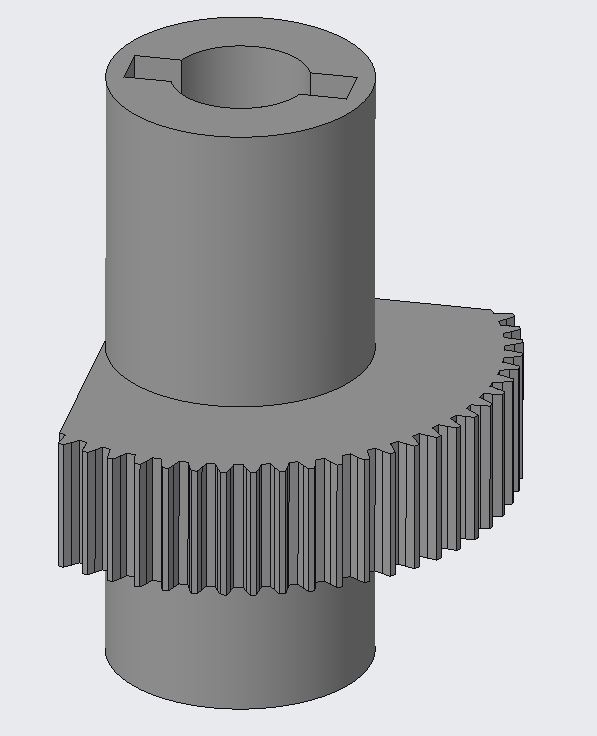
\includegraphics[width=0.4\textwidth]{../../images/Kran/Zahnrad.JPG}
            \caption {Zahnrad}
            \label{fig:et_komponenten}
        \end{figure}


        \subsubsection{Kurvenscheibe}
        Die Kurvenscheibe ist ebenfalls ein 3D-Druckteil. Der Grundkörper ist ein Rohr mit dem Aussendurchmesser 80 mm. An diesem wurden zwei Bahnführungen mittels Freiformflächen für den Kranausleger erzeugt. Die Steigung dieser Flächen ist variabel. Zu Beginn ist die Steigung gering und wird dann exponentiell grösser. Dies wurde aus dem einen Grund gewählt, damit das Anfahren für den Motor nicht zu streng ist. Nachdem die Drehbewegung und der vertikale Hub gemacht wurden, stoppt der Motor und der Kranausleger sollte durch die Schwerkraft heruntergezogen werden. Der Würfel wird nun in der für ihn vorgesehenen Aufnahme auf dem Zug platziert.


        \begin{figure}[H]
            \centering
            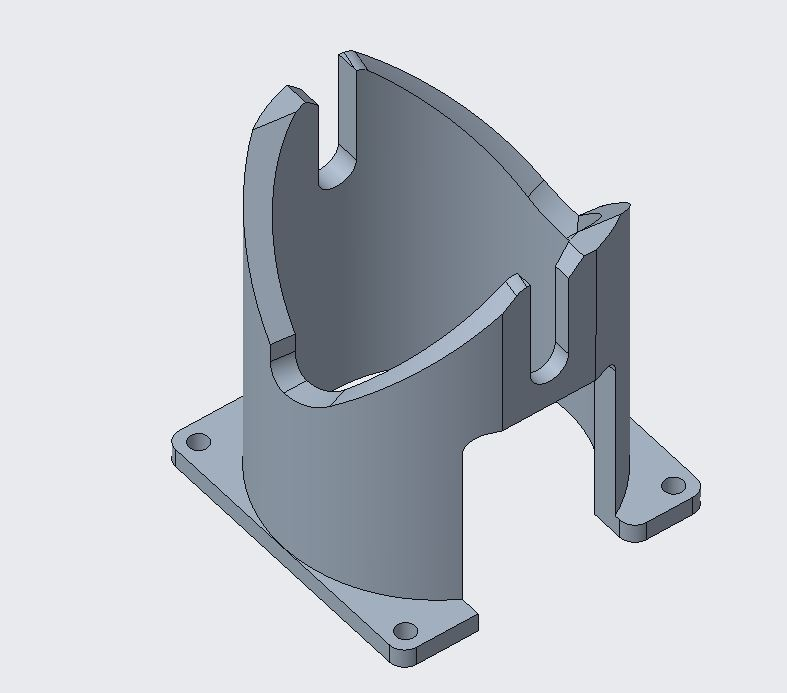
\includegraphics[width=1.0\textwidth]{../../images/Kran/Kurvenscheibe.JPG}
            \caption {Kurvenscheibe}
            \label{fig:et_komponenten}
        \end{figure}




        \subsubsection{Testaufbau}
        Der Testaufbau besteht hauptsächlich aus 3D Druckteilen und weichen Kunststoffen. Er dient momentan als Funktionsmuster und wenn sich dieser weiter bewährt möchte man mit den gefertigten Teilen weiterarbeiten. Der Test dient zur Probe des ausgewählten Lösungskonzepts zur Würfelaufnahme. Erste Tests zeigen, dass die Funktion mit kleinen Anpassungen direkt umgesetzt werden kann.

        \begin{figure}[H]
            \centering
            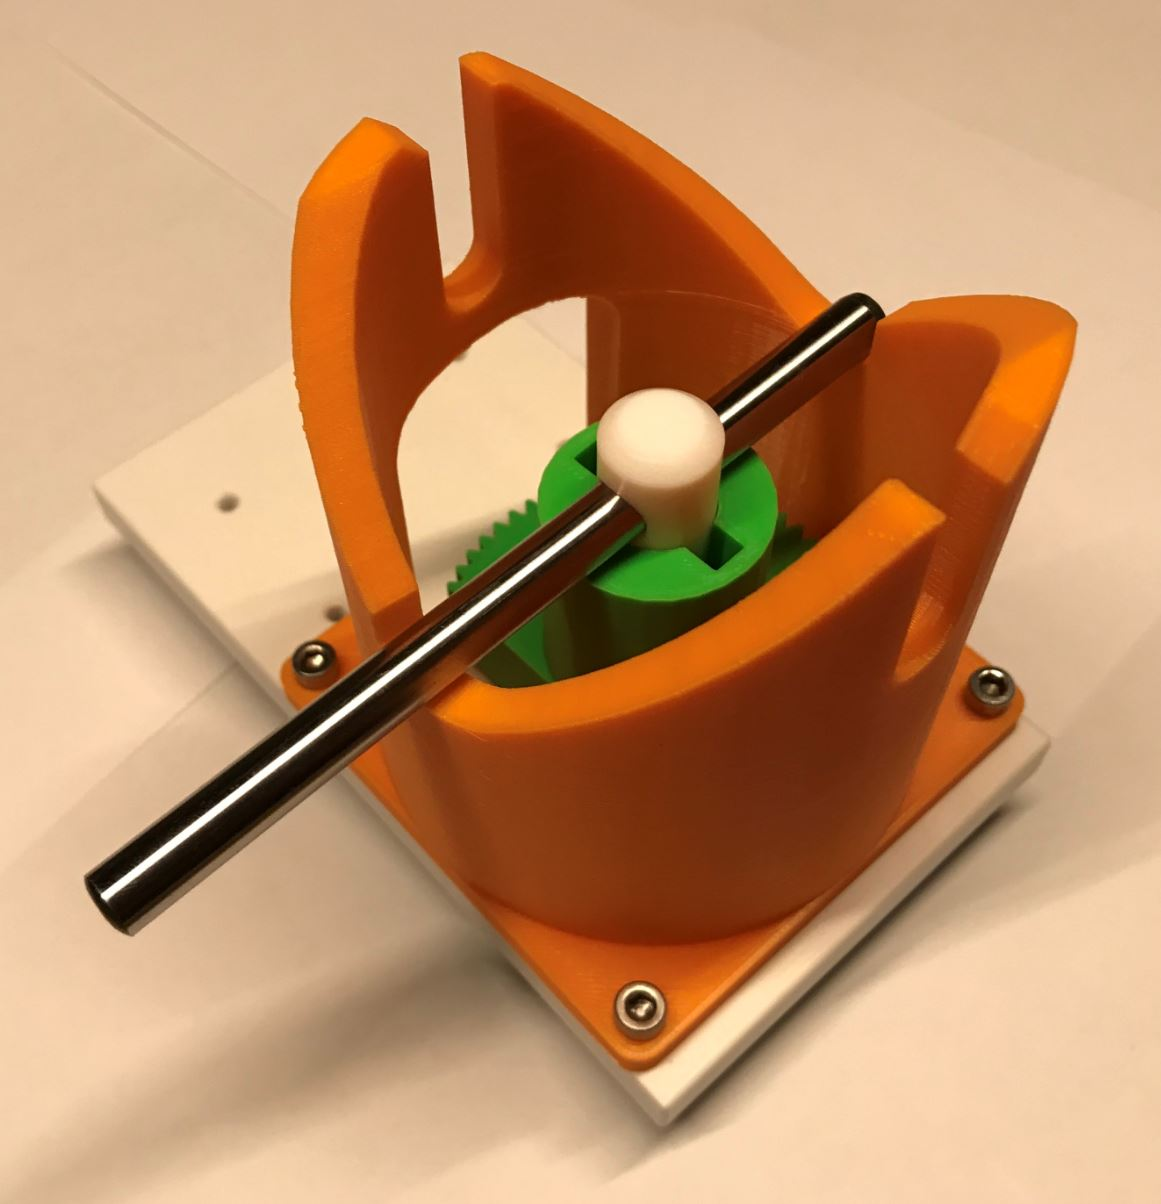
\includegraphics[width=1.0\textwidth]{../../images/Kran/Testaufbau.JPG}
            \caption {Testaufbau}
            \label{fig:et_komponenten}
        \end{figure}


    \subsection{Motorauslegung}
          Um die Aufgabenstellung der schnellen Fahrt auf Schienen Best möglichst zu erfüllen, wird ein zuverlässiger starker Motor benötigt. Um einen solchen aus einer Vielzahl von Auswahlmöglichkeiten zu definieren hat man sich auf den Katalog des maxon motor ag beschränkt. Im Anhang findet man ein Dokument mit den Berechnungen zur Motorauswahl. In Absprache der Disziplinen Elektrotechnik und Maschinentechnik wurde ein bürstenbehafteter Gleichstrommotor als geeignetes Model definiert. Im vorher schon erwähnten Dokument wird für den Gesamten Zug eine Masse von 3 Kilogramm gerechnet und einen Raddurchmesser von 22 mm. Für eine Endgeschwindigkeit von 3 m/s mit den definierten Raddurchmessern wird ergibt sich eine Drehzahl von 2600 1/min. Mit einer Übersetzung von 2 was mit Zahnrädern und den Platzverhältnissen gut realisierbar ist, ergibt sich eine Abgangsdrehzahl für den Motor von 5200 1/min. Das ist im Rahmen der Motoren von maxon motor ag. Was jedoch den Motor an seine Grenzen führt, wird die Grenzbeschleunigung sein. Durch die Beschleunigung entstehen Trägheitskräfte, welche durch ein Moment vom Motor überwunden werden müssen. Das Moment rechnet sich aus der gewollten Beschleunigung, der Masse und dem Hebel auf den Rädern. Wird nun die Übersetzung von 2 noch eingerechnet ergibt sich ein Moment von 110 mNm. Durch die Schienen haben wir eine Leistung zur Verfügung. Diese ergibt sich aus der Spannung 20 Volt und dem Strom von 3 Ampère. 60 Watt stehen also theoretisch zur Verfügung. Für eine preiswerte Lösung in Form eines DC Motors kommen bei maxon motor ag nur die zwei Produktreihen DCX und RE in Frage. Maxon motor ag bietet ein Sponsoring an in Form von Motoren mit kleinen Makeln, die nicht mehr ausgeliefert werden dürfen. Die Wunschmotoren der Gruppe 28 sind auf Grund der Leistung der DCX 32 oder der RE 30.

    \begin{figure}[H]
        \centering
        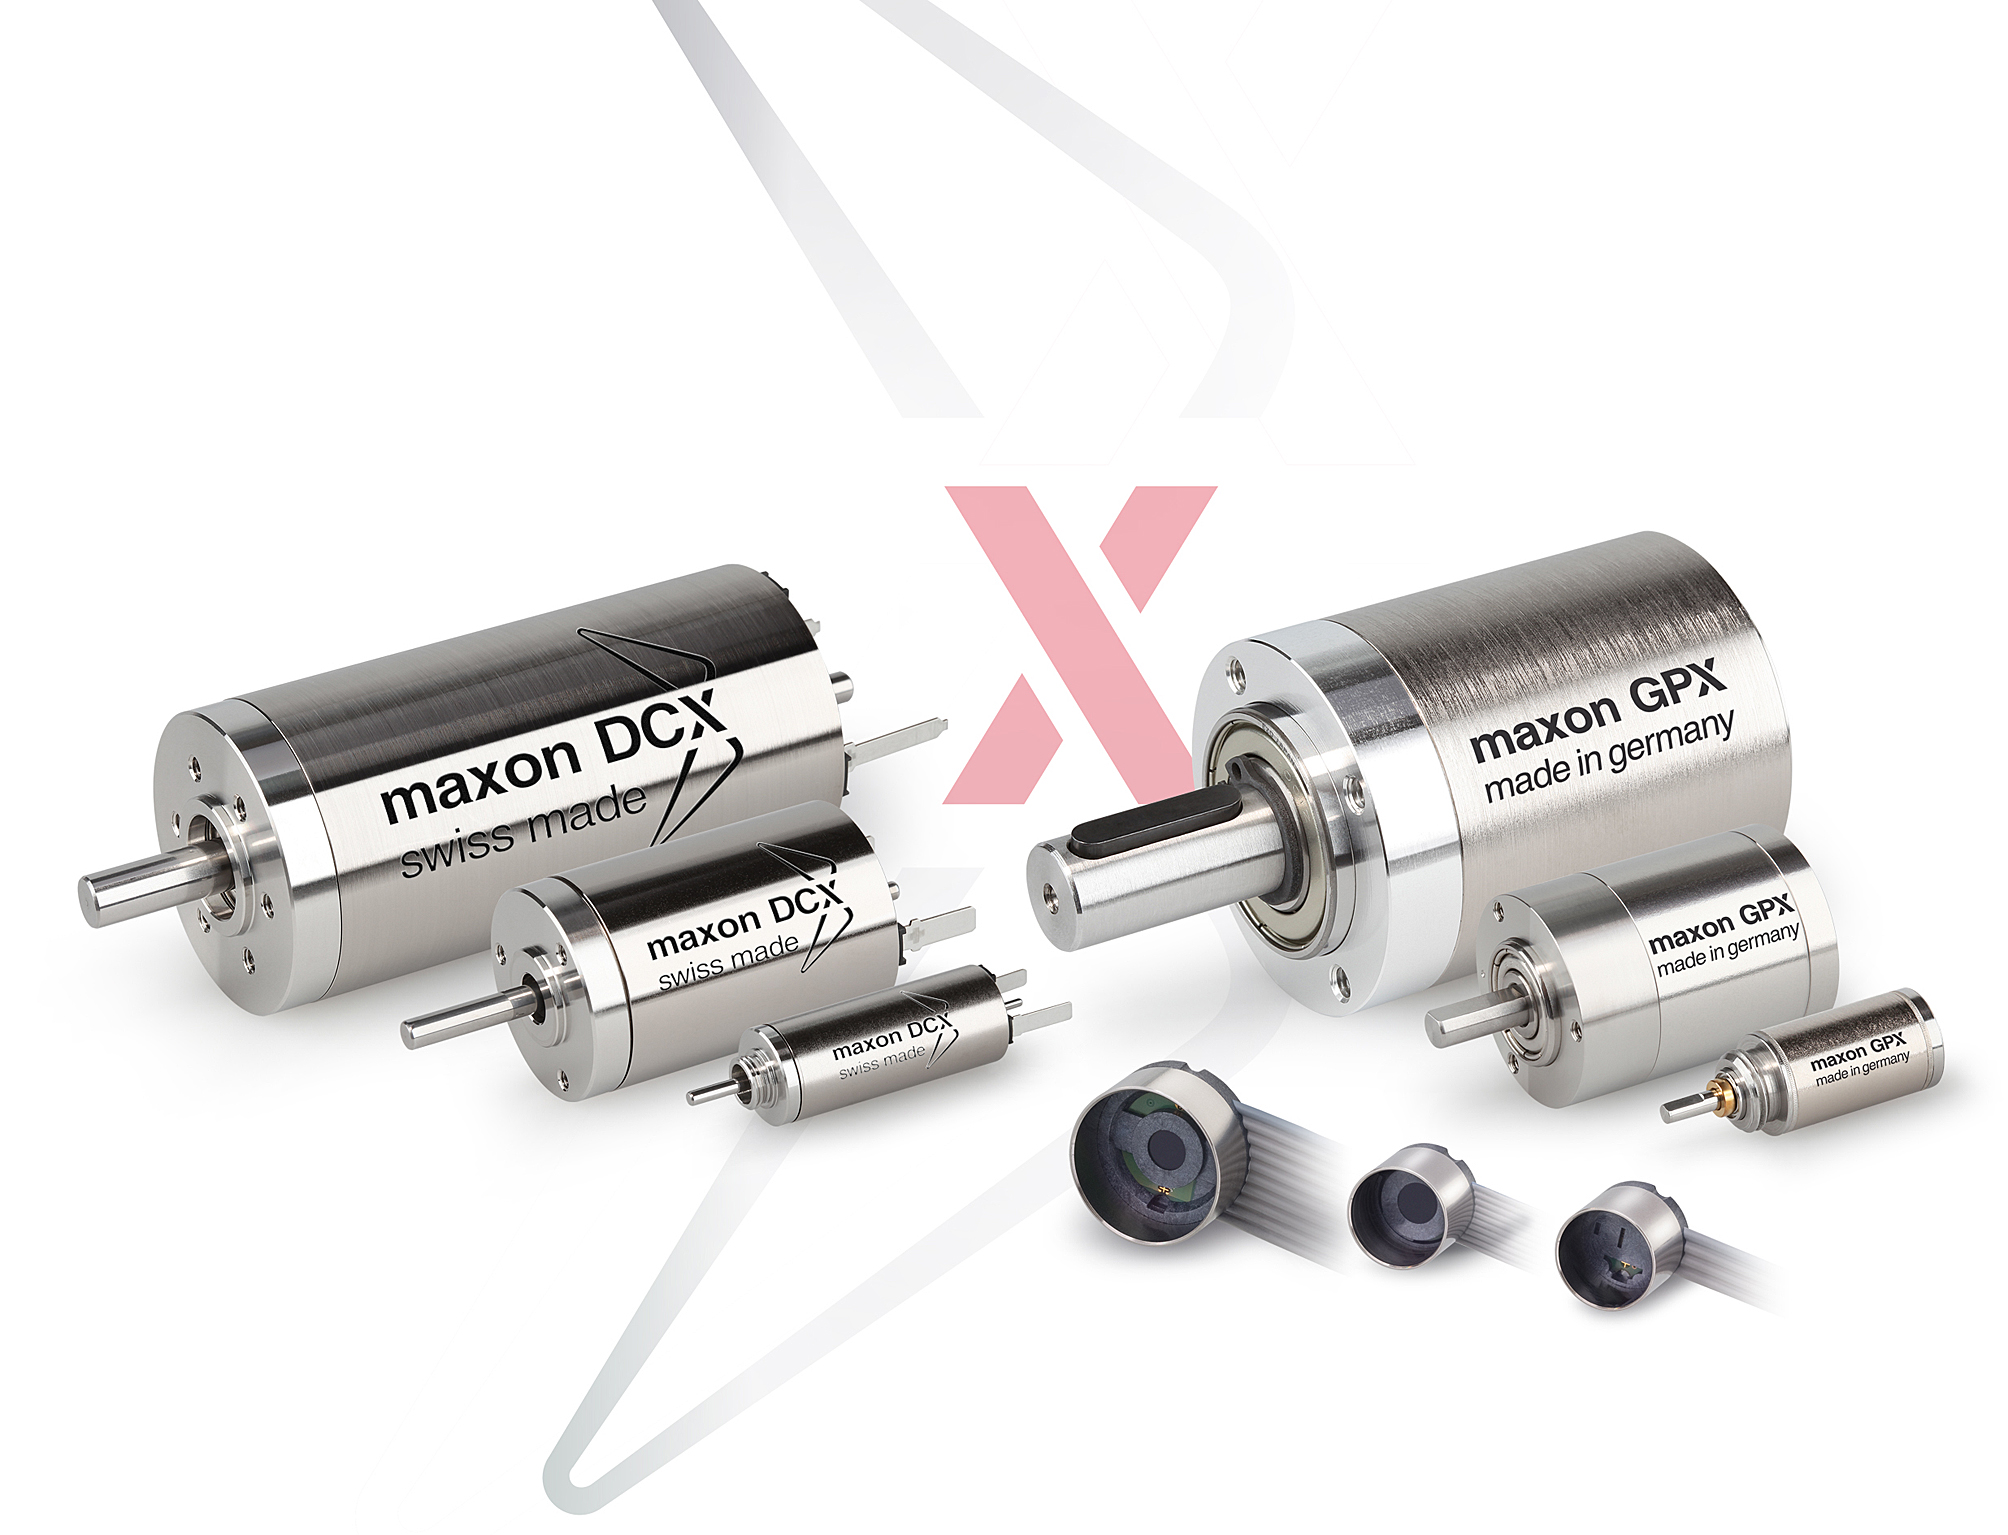
\includegraphics[width=1.0\textwidth]{../../images/Kran/Motors.JPG}
        \caption {DC Motoren}
        \label{fig:et_komponenten}
    \end{figure}


    \end{document}